\chapter{Projekt systemu Soccer Match Predictor}

\noindent Podczas projektowania systemu należało podjąć decyzję na jakie komponenty powinien on zostać podzielony. Poniżej są one krótko scharakteryzowane. Część z nich odpowiada koncepcji pewnego potoku przetwarzania danych charakterystycznego dla inspiracji z rozwiązań niektórych systemów uczących się (z j. ang. tzw. pipeline ML).

Ze względu na różnorodne źródła danych, pierwszym krokiem było połączenie ich w jeden spójny zbiór. Dla efektywnego przechowywania tak zintegrowanych danych zdecydowano się na stworzenie bazy danych Microsoft SQL Server, która jest dostępna na platformie Azure Cloud dla każdego potencjalnego użytkownika. Powyższa baza jest przeniesiona z bazy danych SQLite, ale musiała zostać uzupełniona innymi źródłami danych. W tym celu utworzona została konfigurowalna aplikacja konsolowa.

Kolejną decyzją do podjęcia był transfer danych z przygotowanego źródła do skryptów przygotowujących wybrane cechy dla późniejszego wykorzystania algorytmów uczenia maszynowego. Komponentem do tego wykorzystywanym jest specjalna aplikacja internetowa, utworzona jako web API. Założono, że zapytania do bazy danych powinny zostać wykonane na niezależnym poziomie, aby umożliwić wykorzystanie zasobów platformy Azure Cloud.

W celu rozdzielenia implementacji algorytmów i fazy przygotowywania cech, które otrzymają one na wejściu, powstała biblioteka w utworzona w języku Python. Dzięki temu twórcy algorytmów uczących mogą niezależnie otrzymywać jednolicie przetworzone dane. Równocześnie możliwe jest wykonywanie dodatkowych analiz rozkładów wartości wybranych cech (odpowiedniej tzw. wizualnej eksploracji danych).

Wszystkie te komponenty są zapleczem dla głównego celu systemu, czyli środowiska w którym użytkownik końcowy (np. analityk sportowy) będzie mógł skorzystać z wcześniej przygotowanych danych i algorytmów. Jest nim interaktywny \textit{Jupyter Notebook}, który jest narzędziem do wykonywania predykcji przez utworzone algorytmy.

Architektura systemu na ogólnym poziomie została przedstawiona w postaci schematu na rysunku \ref{fig:arch1}, którego części składowe są następnie wyjaśnione.
\newpage

\section{Ogólny schemat systemu i jego architektura}
\label{arch}
    \begin{figure}[h] 
        \centering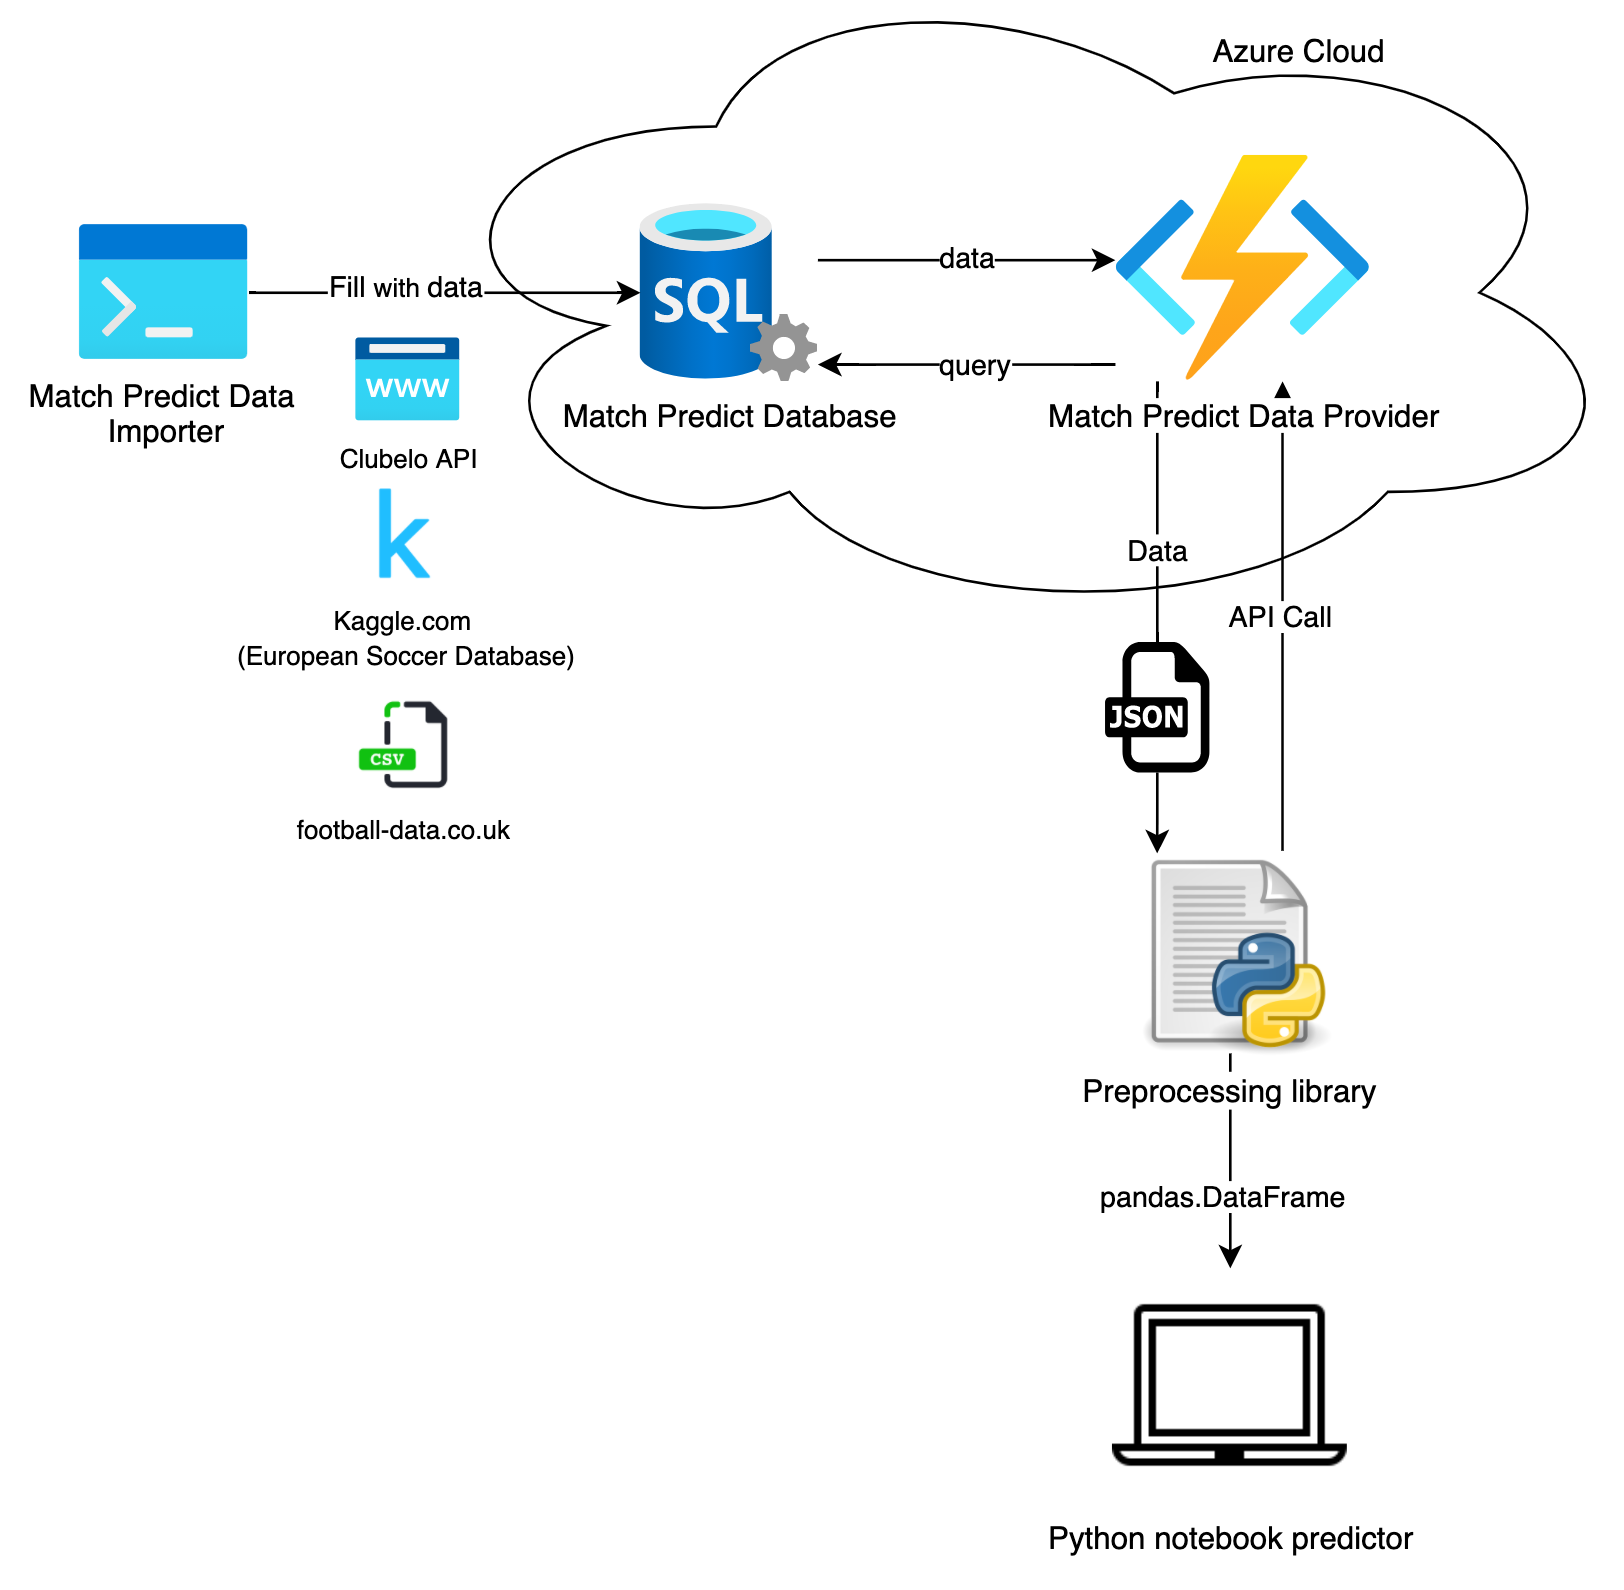
\includegraphics[width=\textwidth]{figures/MatchPredictorArchitecture.png}
        \caption{Architektura systemu Soccer Match Predictor}
        \label{fig:arch1}
    \end{figure}
\newpage

\noindent Pierwszym komponentem jest \textbf{Match Predict Data Importer}, dalej nazywany \definicja{MPDI}. Jest to aplikacja konsolowa napisana w języku C\#, której zadaniem jest import danych z różnych źródeł do docelowej bazy danych widocznej na schemacie jako \textbf{Match Predict Database}.

Baza jest przechowywanym w chmurze Azure komponentem Microsoft SQL Server, w której składowane są wszelkie dane wykorzystywane dalej w systemie. Schemat bazy danych został przedstawiony w sekcji \ref{database_schema}.

Match Predict Data Provider (dalej zwany \definicja{MPDP}) służy w produkcie jako web API, które przesyła dane w formacie JSON. Dane pochodzące z bazy Match Predict Database są odpowiednio agregowane. Komponent ten to aplikacja Azure Function napisana w języku C\#, która również znajduje się w chmurze Azure.

~

Kolejnym komponentem w systemie widocznym na schemacie jako \textbf{Preprocessing library} jest biblioteka służąca do pobierania danych i ich wstępnego przetwarzania wraz z tworzeniem zbioru cech. Jest to moduł napisany w języku Python, który może być wykorzystany w dowolnej aplikacji napisanej w tym języku. Komunikuje się on z opisaną wyżej bazą danych przy pomocy udostępnionego przez nią interfejsu web API i otrzymuje od niego dane w formacie JSON, natomiast korzystającym z niego klientom przekazuje wygodne do operowania dane w formacie \definicja{pandas.DataFrame}. 

Uniwersalność tego modułu polega na tym, że całkowicie ukrywa on szczegóły implementacji swoich operacji pobierania danych z bazy, przetwarzania ich oraz tworzenia cech i udostępnia jedynie metody pozwalające na pobranie danych dla konkretnych sezonów i/lub konkretnych drużyn. Dzięki temu klient korzystający z tego modułu jest niezależny od wszelkich zmian strukturalnych w bazie danych czy interfejsie służącym do komunikacji z nią.

~

Ostatnim elementem jest widoczny na schemacie \textbf{Python notebook predictor}, który pełni rolę środowiska testowe do porównywania różnego rodzaju algorytmów stosując różne podejścia i techniki. Jest to aplikacja stworzona w \textit{Jupyter Notebook}, czyli w rozbudowanym narzędziu uruchamianym w przeglądarce internetowej pozwalającym na m.in. separowanie poszczególnych części kodu i uruchamianie ich niezależnie od siebie. Umożliwia to na przykład jednorazowe pobranie danych na samym początku pracy i wielokrotne użycie ich w późniejszych eksperymentach.

Środowisko to jest klientem opisanego wyżej modułu do wstępnego przetwarzania danych i korzysta z niego do pobierania przetworzonych danych. 

\newpage
\section{Schemat bazy danych}
\label{database_schema}
\begin{figure}[h]
  \centering
   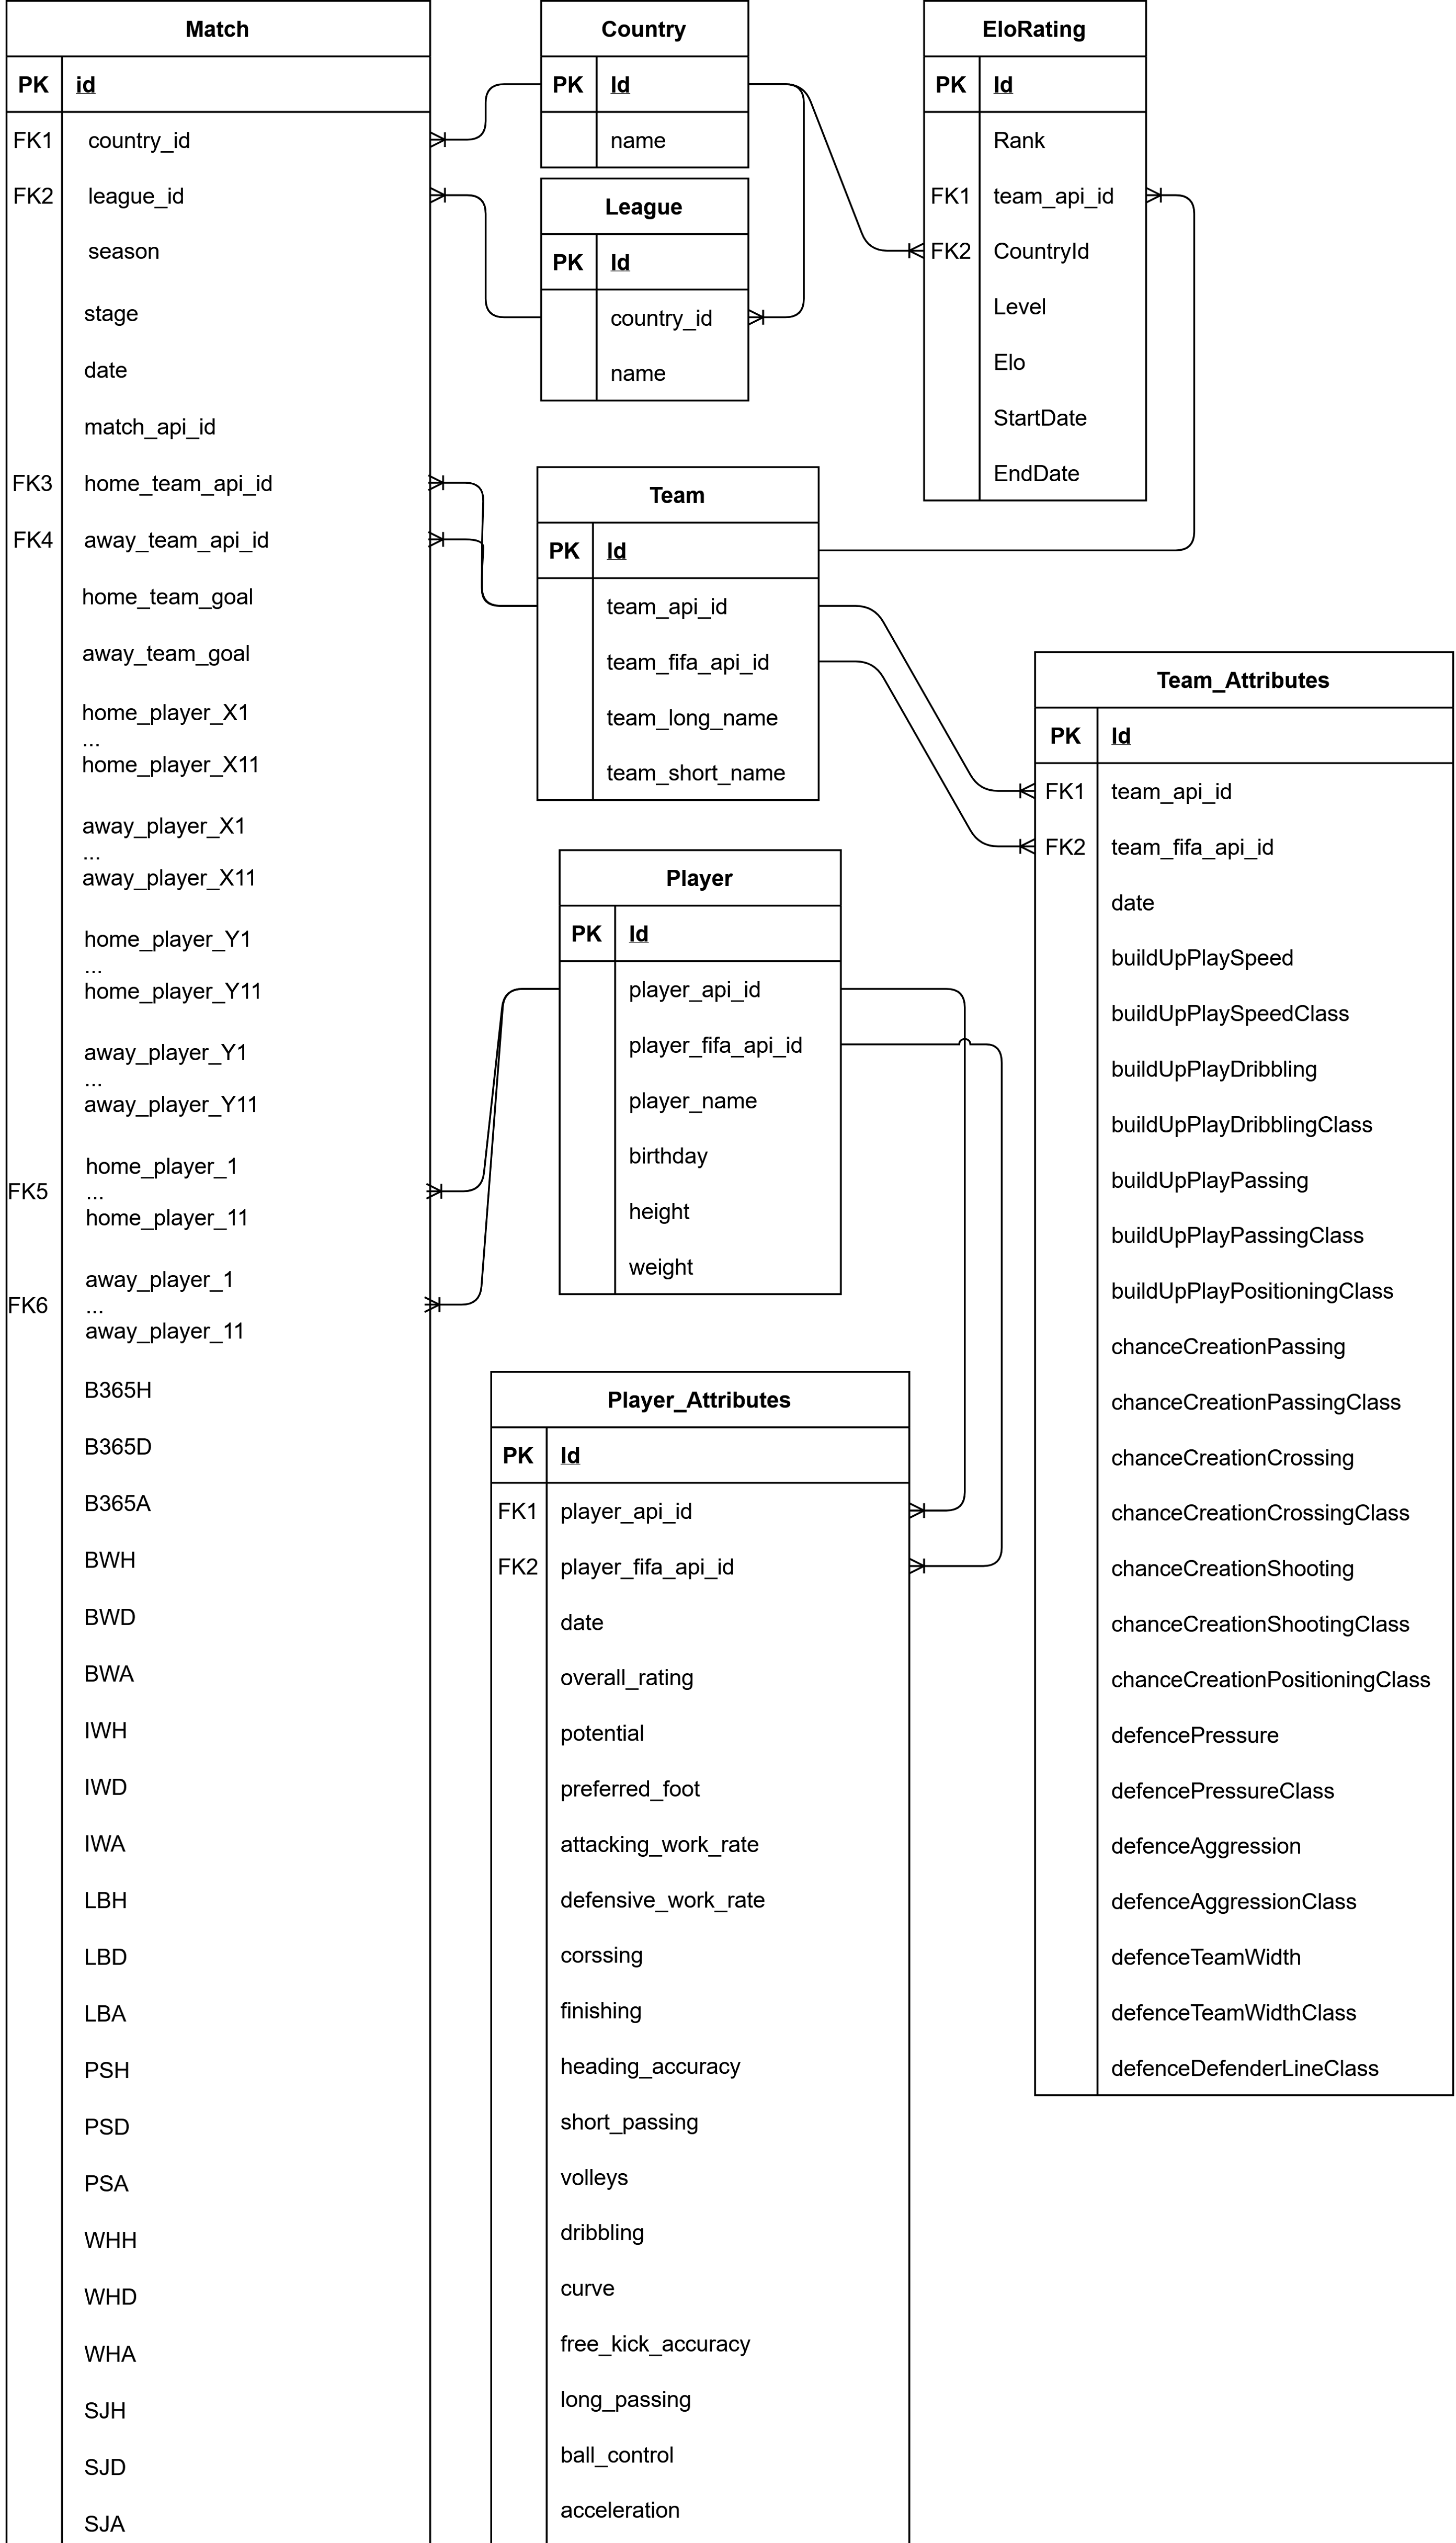
\includegraphics[width=0.83\textwidth]{figures/match_predict_schema_1.png}%

\end{figure}
\newpage
\begin{figure}[h]
\ContinuedFloat
    \centering
  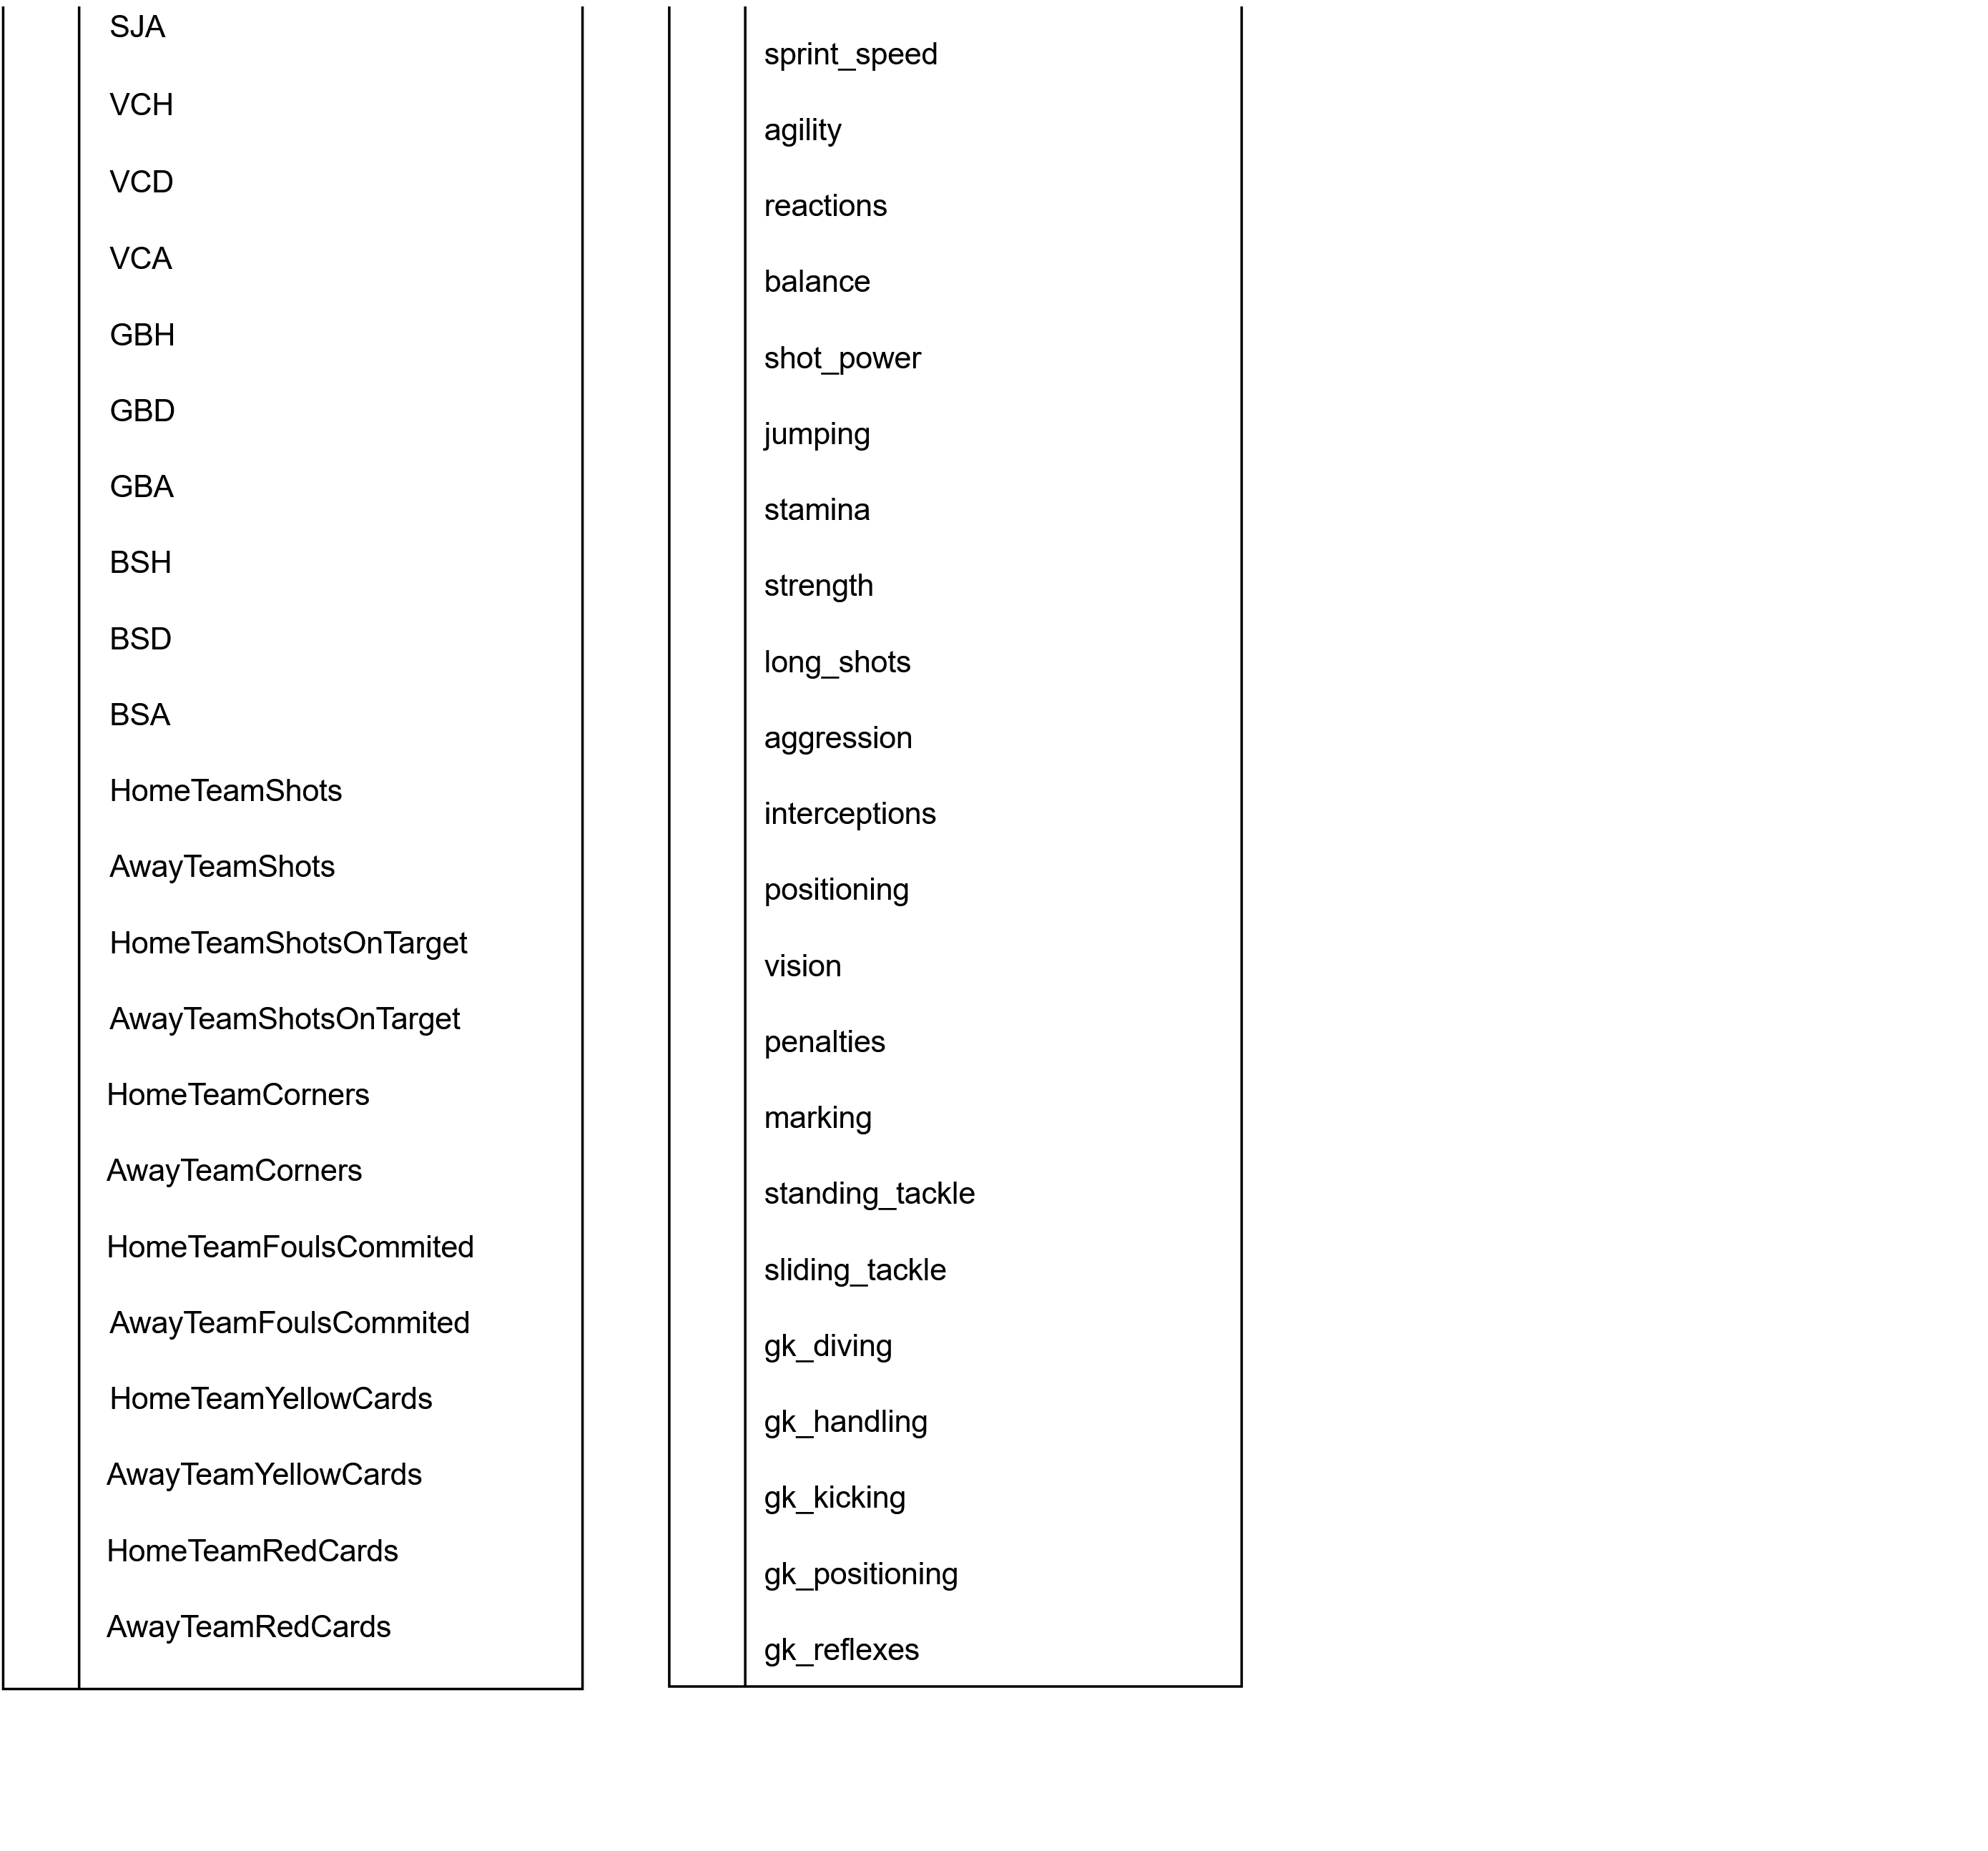
\includegraphics[width=0.83\textwidth]{figures/match_predict_schema_2.png}%
  \addtocounter{figure}{1}
  \caption{Schemat bazy danych \textit{Match Predict}}
    
  \label{fig:match_predict_schema}
    
\end{figure}
 
\noindent Rysunek \ref{fig:match_predict_schema} przedstawia schemat bazy danych \textbf{Match Predict Database} widocznej na rysunku architektury systemu \ref{fig:arch1}. Jest to relacyjna baza danych, stworzona, jak to wcześniej wspomniano w sekcji \ref{arch}, przy użyciu technologii Microsoft SQL Server.

Podstawą dla schematu była pozyskana z strony Kaggle.com baza \textit{European Soccer Database}\footnote{\url{https://www.kaggle.com/hugomathien/soccer}}. Została przekształcona, aby działała w systemie Microsoft SQL Server. Zastosowano odpowiednie filtry, tak aby zawierała dane tylko z interesującej nas ligi angielskiej.

W centrum wszystkich tabel znajduję się tabela \textbf{Match}. Zawiera on dane dotyczące poszczególnych meczów, które zostały rozegrane w latach 2008-2016 w lidze angielskiej. Gdzie: 
\begin{itemize}
    \item Id jest kluczem głównym tabeli, unikatowym identyfikatorem meczu
    
    \item Pola country\_id oraz league\_id są kluczami obcymi do odpowiednich tabel \textbf{Country} oraz \textbf{League}
    
    \item Season oznacza w jakim sezonie został zagrany mecz, zapisane w formacie \{rok\}/\{rok+1\}
    
    \item Stage oznacza numer kolejki ligowej
    
    \item Date to data zagranego meczu
    
    \item Match\_api\_id również jest unikatowym identyfikatorem, znajduję się on w bazie jako id pochodzące ze źródłowego zbioru danych
    
    \item Home/away\_team\_api\_id to klucze obce wskazujące na tabele \textbf{Team}. Odnoszą się one do api\_id, które po raz kolejny są unikalnym identyfikatorem drużyn z oryginalnego źródła danych
    
    \item Home/away\_team\_goal to liczba goli strzelonych przez poszczególne drużyny w trakcie meczu
    
    \item Pola home/away\_player\_X1-11 oraz home/away\_player\_Y1-11 oznaczają pozycje zawodnika na boisku
    
    \item Pola home/away\_player\_1-11 są kluczami obcymi, które odnoszą się do tabeli \textbf{Player}. Zawierają wartości player\_api\_id poszczególnych zawodników biorących udział w rozgrywce
    
    \item Widoczne na schemacie \ref{fig:match_predict_schema} pola zaczynając od B365H do BSA to wartości przedstawiające wysokości kursów, które poszczególne zakłady bukmacherskie oferowały na dany typ zdarzenia. Kolumny kończące się na 'H' wskazują zakład oznaczający wygraną gospodarza, kończące się na 'A' wygraną drużyny gości, a 'D' oznacza kurs na zakłady, które symbolizują remis. Według opisu zbioru danych z serwisu internetowego Kaggle\footnote{\url{https://www.kaggle.com/hugomathien/soccer}}, dane te pochodzą ze strony \url{football-data.co.uk}, gdzie można znaleźć historyczne wartości zakładów bukmacherskich w lidze angielskiej
    
    \item Pola od HomeTeamShots do AwayTeamRedCard w tabeli \textbf{Match} zawierają wszelkie statystyki meczu takie jak strzały na bramkę, faule, ilości żółtych i czerwonych kartek w meczu
\end{itemize}

Tabele \textbf{Country} oraz \textbf{League} zawierają tylko informacje o nazwach odpowiednio kraju oraz ligi. Obecna zawartość tych tabel to pojedyncze wpisy, jednak pozostały w bazie w razie dalszego rozwoju projektu.

Encja \textbf{Team} zawiera nazwy drużyn oraz ich identyfikatory z oryginalnych źródeł danych (team\_api\_id oraz team\_fifa\_api\_id).

Tabela \textbf{Team\_Attributes} jest wypełniona informacjami o statystykach drużyny, które zostały zebrane z corocznych wydań gry FIFA produkowanej przez firmę E.A Games. Autor zestawu danych ze strony \url{www.Kaggle.com} zdobył te dane ze strony internetowej zawierającej te parametry\footnote{\url{https://sofifa.com/}}. Każdy wpis w encji zawiera datę, dzięki której wiemy do którego roku odnosi się danych wpis dla danej drużyny. Klucze obce team\_api\_id oraz team\_fifa\_api\_id są referencją do tabeli \textbf{Team}.

Encja \textbf{Player} posiada podstawowe informacje o poszczególnych zawodnikach takie jak wzrost, rok urodzenia i wagę. Podobnie jak tabela \textbf{Team}, posiada unikalne identyfikatory, które pochodzą z oryginalnych źródeł.

Tak jak w przypadku drużyn, każdy zawodnik posiada zestaw statystyk określających jego poziom w odpowiedniej tabeli o nazwie \textbf{Player\_Attributes}. Zawartość tej encji również została zebrana ze strony internetowej, ma której opublikowano informacje o zawodnikach w corocznych wydania gry FIFA. Dodatkowo posiada datę, określającą rok, dla którego te dane są aktualne. Klucze obce player\_api\_id oraz player\_fifa\_api\_id są referencją do tabeli \textbf{Player}. 

Ostatnią tabelą, która znajduje się na schemacie \ref{fig:match_predict_schema} jest \textbf{EloRating}. Dane w tej tabeli pochodzą ze strony internetowej \url{http://clubelo.com/}, a główną informacją pobieraną z niej to wartość Elo. \definicja{StartDate} oraz \definicja{EndDate} to towarzyszące tej wartości momenty, między którymi była obowiązująca. Rank to miejsce w rankingu danej drużyny, gdzie kryterium jest właśnie \textit{Elo rating}. Team\_api\_id to klucz obcy odnoszący się do tabeli \textbf{Team}, służący do ustalenia, do której drużyny należy dany wpis Elo. CountryId to klucz obcy do encji \textbf{Country}.

Wszystkie tabele mają klucz główny oznaczony jako Id, który jest unikalną liczbą identyfikującą jednoznacznie każdy wpis w poszczególnych tabelach.
\newpage
\section{Opis web API} \label{arch:webApi}
\noindent
Bezpośrednie pobieranie informacji z bazy danych nie byłoby wygodne dla użytkowników. W tym celu utworzone zostało web API nazwane \textbf{Match Predict Data Importer} na schemacie \ref{fig:arch1}. Zaprojektowane w technologii \definicja{Azure Function}\footnote{\url{https://docs.microsoft.com/pl-pl/azure/azure-functions/functions-overview}} i udostępnione w sieci przy pomocy platformy \definicja{Azure Cloud}.

Podczas projektowania systemu zostały ustalone dwa punkty końcowe, których odpowiedzią miały być wstępnie przetworzone dane w formacie JSON.
\begin{itemize}
    \item \textbf{api/Matches/Season/DetailedMatch/\{season\}/\{historicalMatches\}} - funkcja ta zwraca mecze ze szczegółowymi informacjami dla podanego sezonu. Argument \textit{season} określa sezon ligowy. Jest to liczba oznaczająca rok rozpoczęcia się rozgrywek, np. '2010' oznacza sezon '2010/2011'. Drugim parametrem jest \textit{historicalMatches}, który jest liczbą oznaczającą ile przeszłych spotkań dla każdej z drużyn w meczu dodatkowo pobrać. Wszystkie te informacje są zwracane w formacie JSON jako lista zawierająca obiekty nazwane \textbf{DetailedMatchWithHistory}, w których znajdują się szczegóły meczu oraz detale każdej z drużyn i graczy biorących udział w rozgrywce wraz z historycznymi meczami. 
    \item \textbf{api/Matches/Season/DetailedMatch/\{season\}/\{teamId\}/\{historicalMatches\}} - w tej funkcji również zwracane są szczegółowo opisane mecze dla konkretnego sezonu. Jedyną różnicą między tym, a poprzednim punktem końcowym jest parametr \textit{teamId}, określający Id drużyny, dla której chcemy otrzymać spotkania w danym sezonie.
\end{itemize}

\section{Środowisko użytkownika docelowego}
\noindent
Jak wspomniano wcześniej, aplikacja jest tworzona dla osób chcących wziąć udział w zakładach bukmacherskich. Przede wszystkim kierowana jest do analityków oraz statystyków konkretnych drużyn, które muszą sprawdzić aktualną formę swojego zespołu oraz porównać ją z przeciwnikiem. Ponadto na podstawie tego oraz otrzymanego przewidywanego wyniku mogą określić taktykę na nadchodzący mecz. Takie informacje są niezbędne przed meczem, a nie w jego trakcie lub po końcowym gwizdku. Dzięki posiadaniu takich danych można dobrać odpowiednią taktykę, zmienić skład wyjściowy czy zastosować jeszcze inne modyfikacje w celu maksymalizacji szansy na wygraną. Jednak, jak powszechnie wiadomo, nie każdy posiada zdolności programistyczne. Założyliśmy, że analitycy sportowi, jak i osoby interesujące się użytkowaniem różnych narzędzi programistycznych, będą potrafiły skorzystać z przygotowanego środowiska do pozyskiwania odpowiedzi od zbudowanego systemu dla konkretnych zapytań. Nie jest tu potrzebna zdolność programowania np. w języku Python, a jedynie wymagana jest wiedza jak załadować i otworzyć dany interfejs (jeśli potencjalny użytkownik nie wyrazi chęci instalacji \definicja{Jupyter Notebook} na swoim komputerze, istnieje wiele różnych środowisk internetowych, które można bezpłatnie wykorzystywać, w tym ładować odpowiednie pliki i uruchamiać dane skrypty. Jednym z nich jest popularna platforma chmurowa \definicja{Google colab}). 

Interfejs użytkownika obejmuje następujące możliwości oraz tryby współpracy z użytkownikiem:
\begin{figure}[H] 
        \centering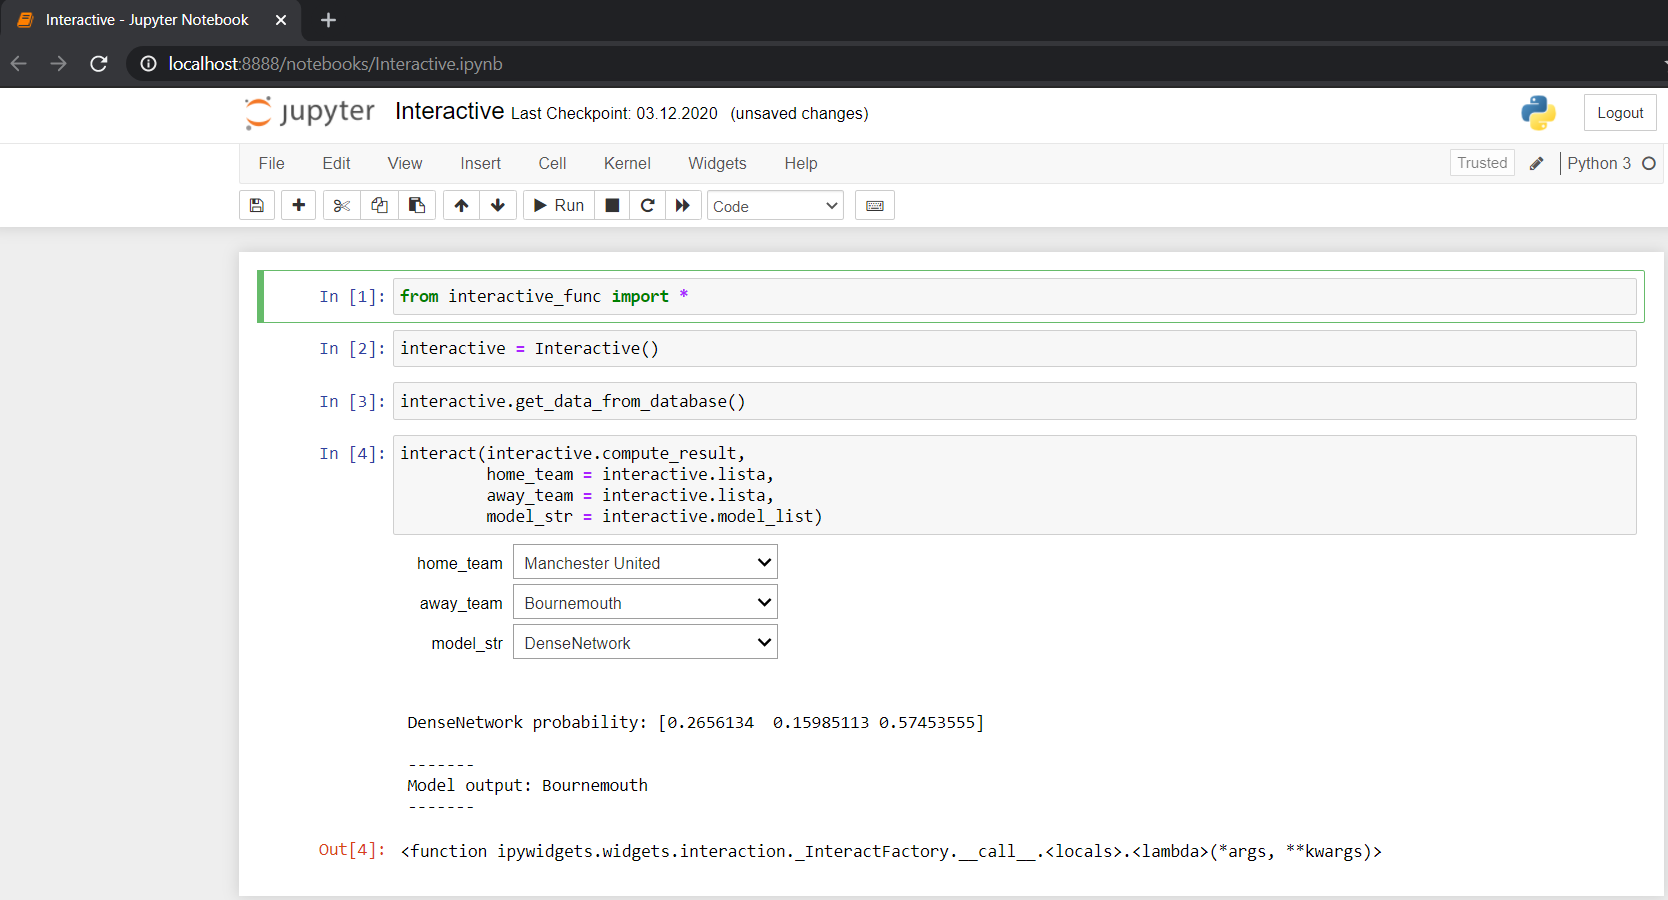
\includegraphics[width=16cm,height=10cm]{figures/Interactive_overview.png}
        \caption{Interaktywny notebook}\label{interactive}
\end{figure}
Do rozpoczęcia pracy z środowiskiem potrzebne jest uruchomienie czterech przedstawionych powyżej komórek programu, a funkcje, które zostaną dzięki temu wykonane, zadbają o to by użytkownik mógł bez pisania jakiegokolwiek kodu pobrać wymagane dane a następnie dokonać predykcji.

Wybór drużyn odbywa się poprzez wybór z rozwijanego menu:
\begin{figure}[H] 
        \centering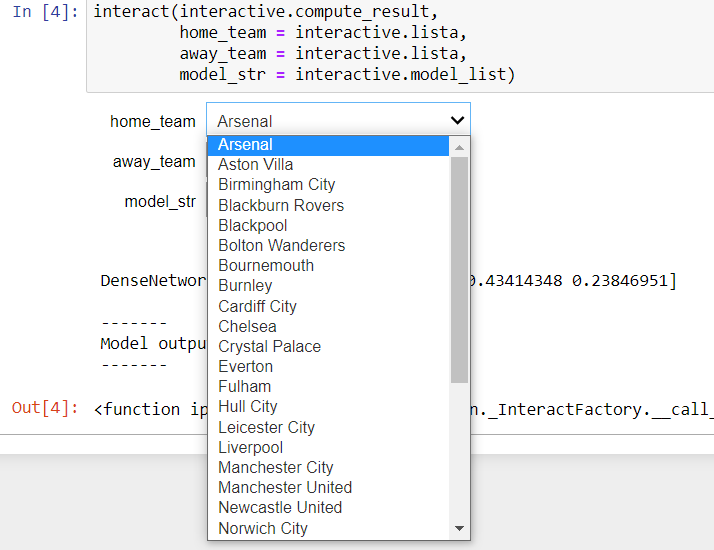
\includegraphics[width=10cm,height=8cm]{figures/Interactive_team_selection.png}
        \caption{Interaktywny wybór drużyn}\label{interactive_tem}
\end{figure}
Dodatkowo pozwala się użytkownikowi na wybór preferowanego przez niego algorytmu, za pomocą którego zwrócony zostanie wynik predykcji:
\begin{figure}[H] 
        \centering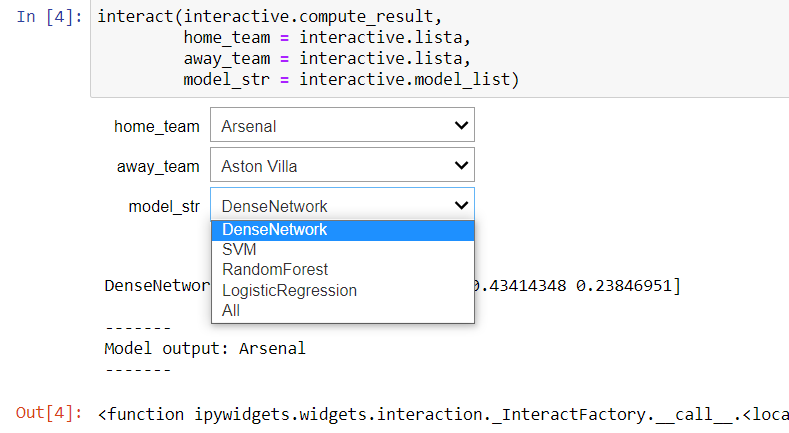
\includegraphics[width=12cm,height=8cm]{figures/Interactive_alg_selection.png}
        \caption{Interaktywny wybór algorytmu}\label{interactive_alg}
\end{figure}
Kiedy użytkownik wyraziłby chęć wykorzystania wszystkich algorytmów, zostaje mu udostępniona taka możliwość i na zasadzie głosowania większościowego (klasa, które uzyska większość głosów zostaje zwrócona, w przeciwnym wypadku gdy udzielenie jednoznacznej odpowiedzi jest niemożliwe, zwracany jest odpowiedni komunikat - rysunek \ref{fig:Resultsb} ) użytkownik jest w stanie uzyskać wynik. W przypadku algorytmów, które zwracają rozkład prawdopodobieństwa przynależności do konkretnych klas wynikowych, również ta informacja jest zwrócona (rysunek \ref{fig:Resultsa}) i wyświetlona dla użytkownika, w celu pokazania mu czy dany wynik jest bardziej lub mniej pewny według wybranego algorytmu. 

\begin{figure}[H]%
    \centering
    \subfloat[\centering
    \label{fig:Resultsa}Wynik wraz z prawdopodobieństwem]{{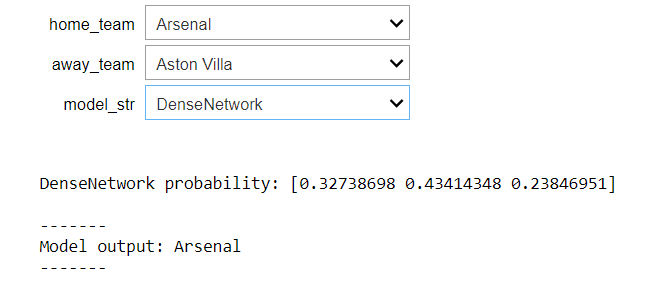
\includegraphics[width=6cm,height=5cm]{figures/Interactive_results.png} }}%
    \qquad
    \subfloat[\centering \label{fig:Resultsb} Brak wyniku dominującego]{{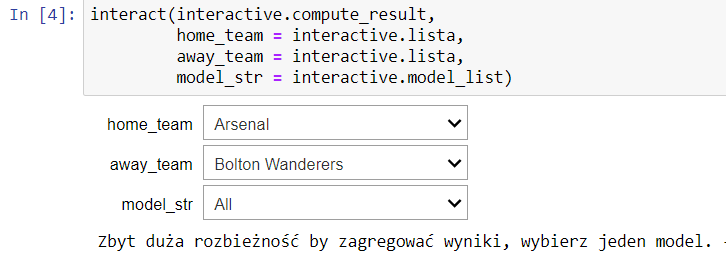
\includegraphics[width=8cm,height=5cm]{figures/Interactive_results2.png} }}%
    \caption{Otrzymywane odpowiedzi zwrotne}%
    \label{fig:Results}%
\end{figure}
Podsumowując, interaktywny notebook jest bardzo prostym, lecz zarazem intuicyjnym interfejsem, który każdy może z powodzeniem wykorzystać, aby odczytać wyniki na podstawie nauczonych modeli predykcyjnych.

\newpage\null\thispagestyle{empty}\newpage